% !TeX root = ../../Parte3.tex
\secmeme{js/semicolon}
\section{Primi passi}
\begin{frame}[fragile]{Messaggi}\transfade\centering
  \begin{enumerate}
    \item Finestre di dialogo (per l'utente):
      \begin{columns}
        \begin{column}{.5\textwidth}
          \begin{minted}{js}
alert("Ciao!");
          \end{minted}
        \end{column}
        \begin{column}{.5\textwidth}\centering
          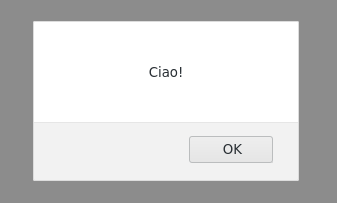
\includegraphics[width=.6\columnwidth]{img/alert}
        \end{column}
      \end{columns}
    \item Stampa nella consolle (per debug):
    \begin{columns}
      \begin{column}{.5\textwidth}
        \begin{minted}{js}
console.log("Ciao!");
          \end{minted}
        \end{column}
        \begin{column}{.5\textwidth}
          \begin{minted}{sh}
Ciao!
>
          \end{minted}
        \end{column}
      \end{columns}
  \end{enumerate}
\end{frame}

\begin{frame}[fragile]{Variabili}\transfade\centering
  \begin{minted}{js}
// Dichiarazione
var pippo; // variabile globale: sconsigliato usarle
let pluto; // variabile locale

// Assegnamento
pluto = 20;

// Dichiarazione con inizializzazione
let paperino = "duck";

// Costanti (obbligatria inizializzazione)
const TOPOLINO = 1.5;

// Utilizzo
pluto = 7 * (TOPOLINO + pluto % 6) / 2**3 - 1;
//      7 · ( 1.5     +  20 mod 6) ÷  2³  - 1
alert(pluto);  // 2.0625
  \end{minted}
  \pause
  \alert{Attenzione!} Usare varibili non dichiarate non da errore, ma non va fatto!!!\\
  Inserire nella prima riga \mintjs[bgcolor=mintbg]{"use strict";} per evitare questo ed altri errori.\\
\end{frame}

\begin{frame}[fragile]{Stringhe}\transfade\centering
  \begin{minted}[fontsize=\normalsize]{js}
let a = "Questa è una stringa";
let b = 'Questa è una stringa';
let c = 'Questa è una "stringa"';

let pippo = 15;
let d = "Il totale è " + pippo + " euro"; // concatenazione
let e = `Il totale è ${pippo} euro`; // interpolazione
  \end{minted}
  \bigskip
  Come scrivere l'accento grave (\texttt{\`}):
  \begin{description}
    \item[Linux] \texttt{AltGr} + \texttt{\'}
    \item[Windows\footnote{Dal tastierino numerico.}] \texttt{Alt} + \texttt{96}
    \item[macOS\footnote{In alcuni computer potrebbe essere necessario digitare uno spazio dopo questa combinazione di tasti.}] \texttt{AltGr} + \texttt{\textbackslash} o \texttt{AltGr} + \texttt{9}
  \end{description}
\end{frame}


\secmeme{js/array}
\subsection{Array}
\begin{frame}[fragile]{Array}\transfade\centering
  \begin{tikzpicture}[scale=0.9, every node/.style={scale=0.9},array/.style={matrix of nodes,nodes={draw, minimum size=7mm, fill=red!40!gray!30!white},column sep=-\pgflinewidth, row sep=0.5mm, nodes in empty cells,
    row 1/.style={nodes={draw=none, fill=none, minimum size=5mm}},
    row 1 column 1/.style={nodes={draw}}}]

    \matrix[array] (array) {
    0 & 1 & 2 & 3 & 4 & 5 & 6 & 7 & 8 & 9\\
      &   &   &   &   &   &   &   &   &  \\};
    \node[draw, fill=gray, minimum size=4mm] at (array-2-9) (box) {};

    \begin{scope}[on background layer]
    \fill[red!40!gray!10!white] (array-1-1.north west) rectangle (array-1-10.south east);
    \end{scope}

    \draw[<-] (array-1-1.north)--++(90:3mm) node [above] (first) {Primo indice};
    \draw[<-] (array-1-10.east)--++(0:3mm) node [right]{Indici};
    \node [align=center, anchor=south] at (array-2-9.north west|-first.south) (8) {Elemento\\ @ indice 8};
    \draw[->] (8)--(box);
    %
    \end{tikzpicture}
    \pause\bigskip
    \begin{minted}[fontsize=\normalsize]{js}
  let a = Array(10); // Array di 10 elementi
  let b = [1, 'a', 1.0]; // Array vuoto
  let c = []; // Array vuoto

  a[8] // elemento inposizione 8 (il nono) di a
> a[8];
  undefined
    \end{minted}
\end{frame}
\begin{frame}[fragile]{Operare con gli array}\transfade\centering
    \begin{minted}{js}
> let a = [];
  []
> a.length;       // Numero di elementi
  0
> a.pushback(12); // Inserisci un elemento
> a;
  [12]
> a.length;
  1
> a.pushback('a');
> a;
  [12, 'a']
> a.length;
  2
> a[0] = 3;       // Modifica elemento
> a;
  [3, 'a']
> a.length;
  2
    \end{minted}
\end{frame}


\secmeme{js/js_aspirina}
\subsection{Oggetti}
\begin{frame}[fragile]{Oggetti}\transfade\centering

\end{frame}